% !TEX root = ../main.tex

%----------------------------------------------------------------------------------------
% APPENDIX A
%----------------------------------------------------------------------------------------
\chapter{PDF Abgaben}
\label{AppendixA}

\textbf{A.1 Zeitplan\\
A.2 Aufgabenstellung\\
A.3 Verwendete Tools\\
A.4 Flankenerkennung Bits für Startdelimiter\\
A.5 Manchester Decoding State Machine\\
A.6 Schemata\\
A.7 Stückliste
}


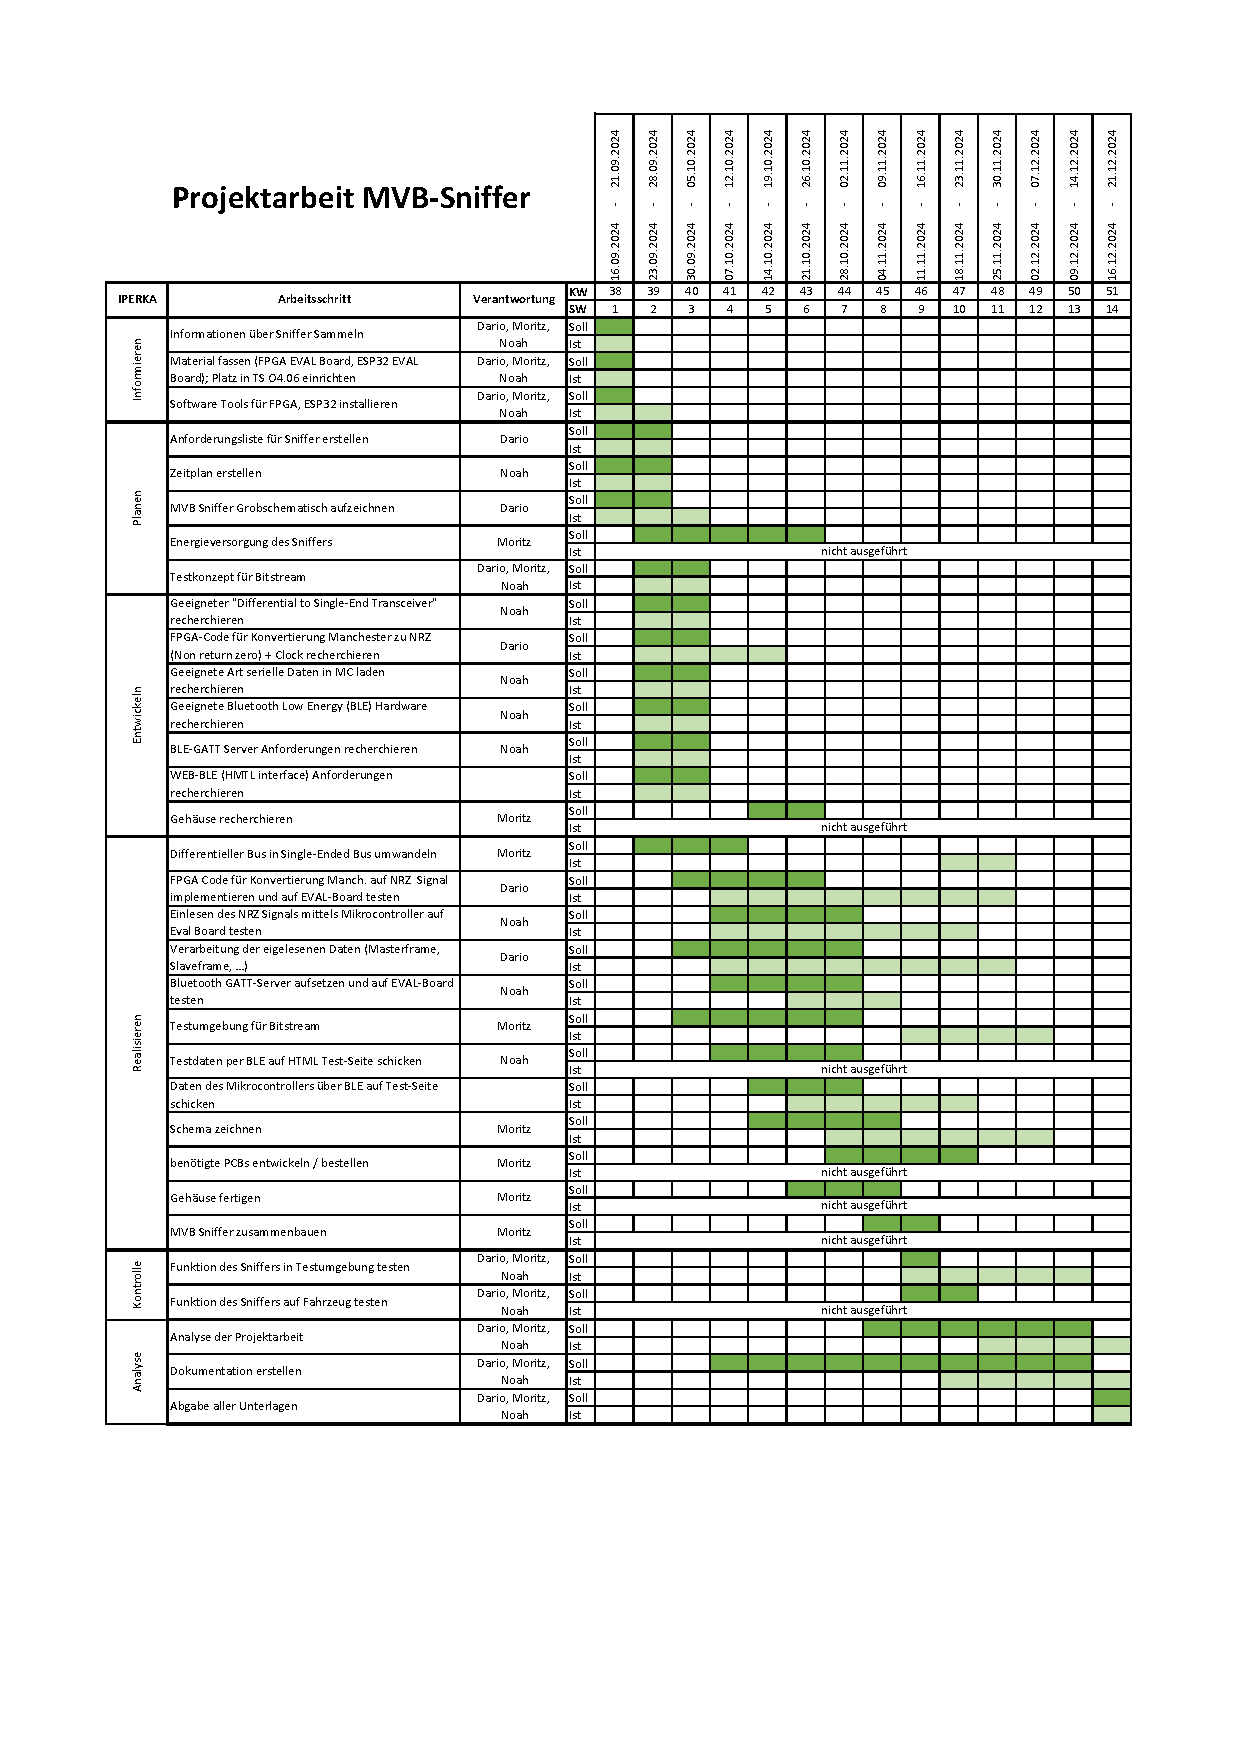
\includepdf[pages=1,pagecommand={\thispagestyle{headings} \section{Zeitplan} \label{app:Zeitplan}}, scale=0.9]{Appendices/Zeitplan.pdf}

\newpage

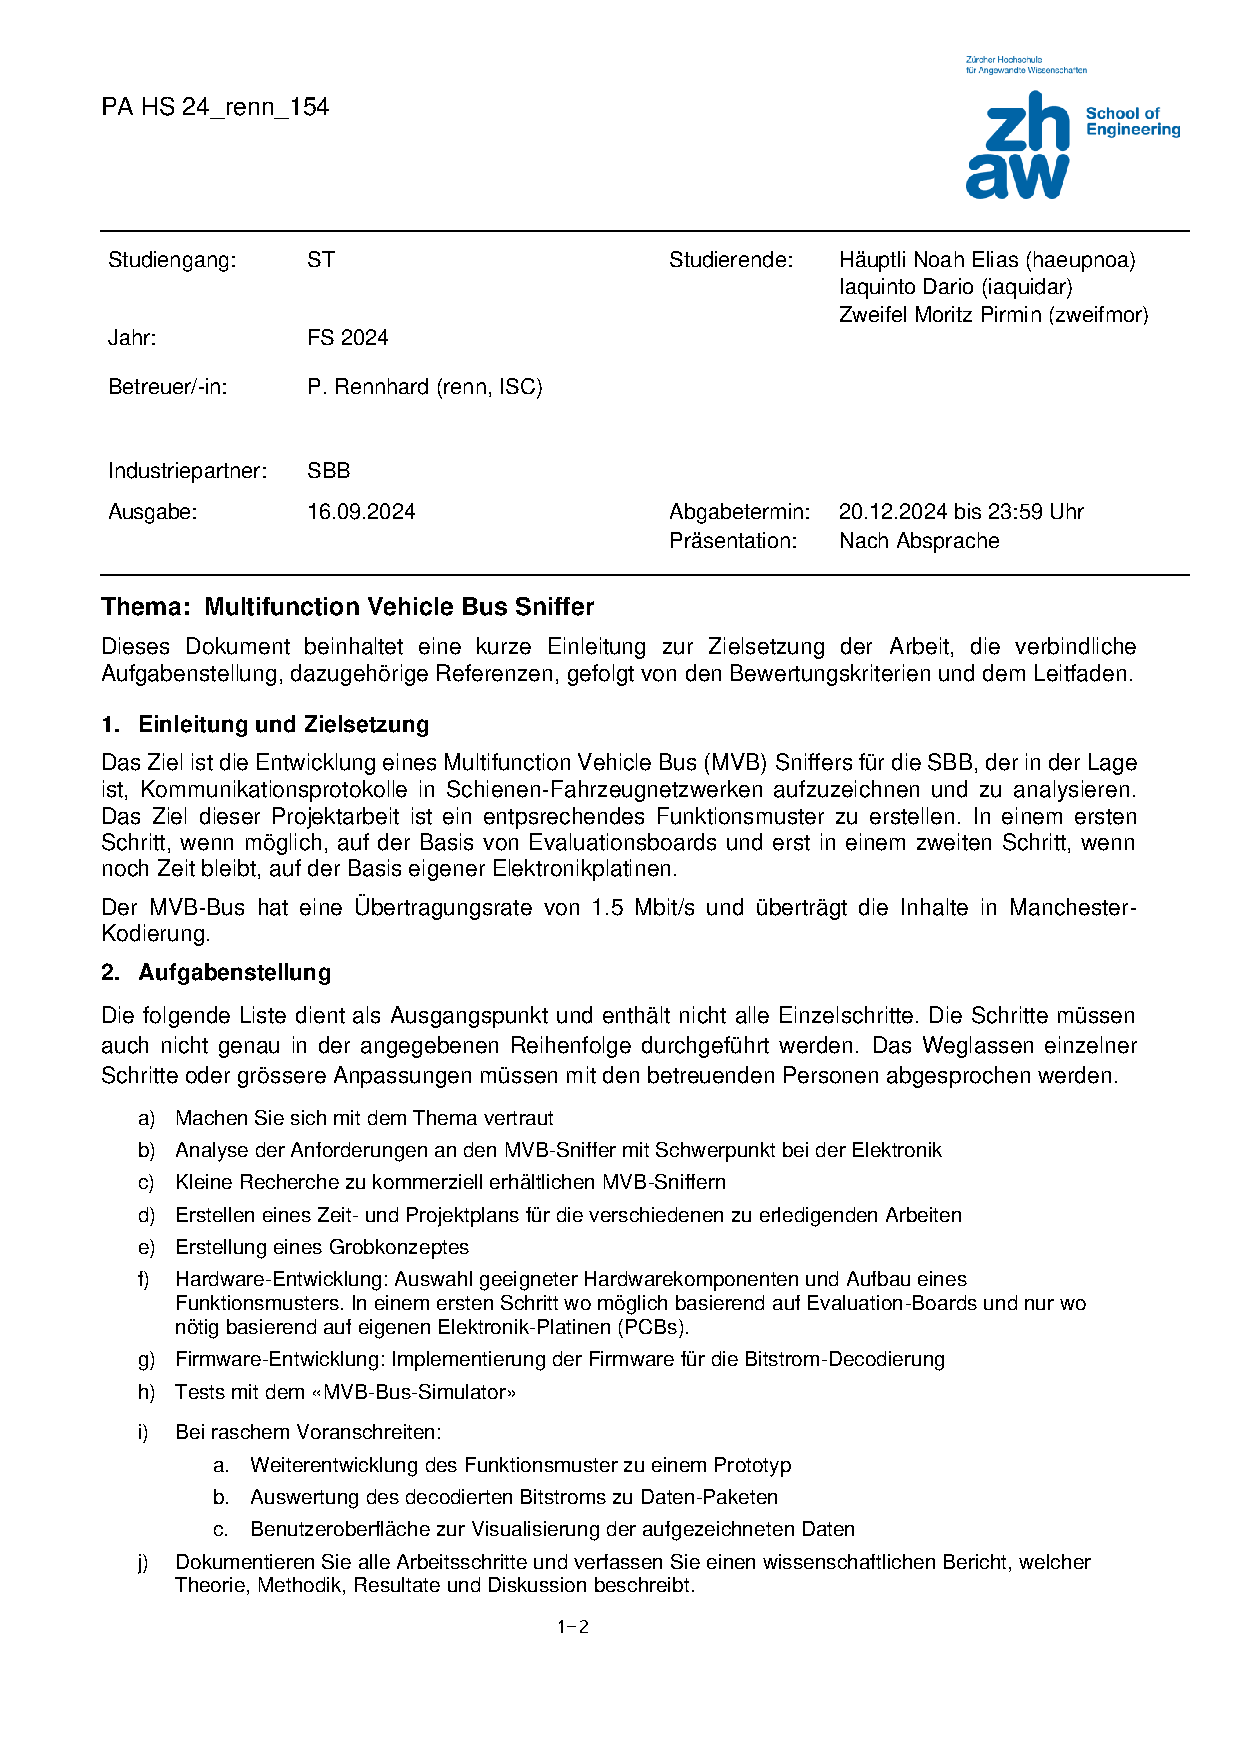
\includepdf[pages=1,pagecommand={\thispagestyle{headings} \section{Aufgabenstellung} \label{app:Aufgabenstellung}}, scale=0.8]{Appendices/PA_renn_Multifunction Vehicle Bus Sniffer_V1.pdf}


\includepdf[pages=2,pagecommand={\thispagestyle{headings}}, scale=0.8]{Appendices/PA_renn_Multifunction Vehicle Bus Sniffer_V1.pdf}



% For referencing this appendix elsewhere, use \ref{AppendixA}
%

%\section{How do I change the colors of links?}
%
%The color of links can be changed to your liking using:
%
%{\small\verb!\hypersetup{urlcolor=red}!}, or
%
%{\small\verb!\hypersetup{citecolor=green}!}, or
%
%{\small\verb!\hypersetup{allcolor=blue}!}.
%
%\noindent If you want to completely hide the links, you can use:
%
%{\small\verb!\hypersetup{allcolors=.}!}, or even better: 
%
%{\small\verb!\hypersetup{hidelinks}!}.
%
%\noindent If you want to have obvious links in the PDF but not the printed text, use:
%
%{\small\verb!\hypersetup{colorlinks=false}!}
%
%\section{How can I add a Figure in the Appendix?}
%
%You can refer to a figure in the Appendix (like \ref{fig:appendix-figure}) and it will show up as expected.
%
%\begin{figure}
%\includegraphics[width=0.25\textwidth]{../Figures/Bart_Simpson.png}
%\centering
%\caption[A random appendix figure]{Bart Simpson. (2023, May 17). In Wikipedia. \url{https://en.wikipedia.org/wiki/Bart_Simpson}}
%\label{fig:appendix-figure}
%\end{figure}


\newpage  % Fügt einen Seitenumbruch ein

\section{Verwendete Tools}
\label{app:VerwendeteTools}

% \begin{table}[H]
%     \centering
%     %\begarin{tabular}{p{2.5cm}p{2cm}p{8.5cm}}
%     \begin{tabular}{>{\raggedright\arraybackslash}p{3cm} >{\raggedright\arraybackslash}p{2cm} >{\raggedright\arraybackslash}p{8cm}}
%     \toprule
%         Programm & Version & Downloadlink\\
%     \midrule
%         ESP-IDF & v5.1.1 & https://github.com/espressif/\mbox{esp-idf}\allowbreak/tree/v5.1.1\\ \hline
%         Visual Studio Code & 1.96.0 & https://code.visualstudio.com/docs/\\  \hline
%         ESP-IDF \mbox{Extension for} VS Code & 1.9.0 & https://marketplace.visualstudio.com\allowbreak/items?itemName=espressif.esp-idf-extension\\  \hline
%         PicoScope 7 TM & 7.1.21.18179 & https://www.picoauto.com/downloads\\ \hline
%         Altium Designer & 24.9.1 (Build 31) & https://www.altium.com/de/products\allowbreak/downloads \\  \hline
%         Intel® Quartus® Prime Lite Edition Software & 23.1.1 & https://www.intel.com/content/www/us\allowbreak/en/software-kit/825278/intel-quartus-prime-lite-edition-design-software-version-23-1-1-for-windows.html\\ \hline
%         Matlab & R2023\_a & von Hochschule bereitgestellt \\ \hline
%         ArbExpress & 3.6 & von Betreuungsperson bereitgestellt \\ \hline
%         Python & 3.10.7 & https://www.python.org/downloads/ \\\hline
%         Bluetility & 1.5.1 & https://github.com/jnross/Bluetility \\
%     \bottomrule
%     \end{tabular}
%     \caption{Verwendete Software-Tools}
%     \label{tab:UsedTools}
% \end{table}


\begin{table}[H]
    \centering
    \begin{tabular}{>{\raggedright\arraybackslash}p{6cm} || >{\raggedright\arraybackslash}p{4cm} || >{\raggedright\arraybackslash}p{3cm}}
    \toprule
        Programm & Version & Downloadlink\\
    \midrule
        ESP-IDF & 5.1.1 & \href{https://github.com/espressif/esp-idf/tree/v5.1.1}{Link} \\ \hline
        Visual Studio Code & 1.96.0 & \href{https://code.visualstudio.com/docs/}{Link} \\ \hline
        ESP-IDF \mbox{Extension for} VS Code & 1.9.0 & \href{https://marketplace.visualstudio.com/items?itemName=espressif.esp-idf-extension}{Link} \\ \hline
        PicoScope 7 TM & 7.1.21.18179 & \href{https://www.picoauto.com/downloads}{Link} \\ \hline
        Altium Designer & 24.9.1 (Build 31) & \href{https://www.altium.com/de/products/downloads}{Link} \\ \hline
        Intel® Quartus® Prime Lite Edition Software & 23.1.1 & \href{https://www.intel.com/content/www/us/en/software-kit/825278/intel-quartus-prime-lite-edition-design-software-version-23-1-1-for-windows.html}{Link} \\ \hline
        Matlab & R2023\_a & von Hochschule bereitgestellt \\ \hline
        ArbExpress & 3.6 & von Betreuungsperson bereitgestellt \\ \hline
        Python & 3.10.7 & \href{https://www.python.org/downloads/}{Link} \\ \hline
        Bluetility & 1.5.1 & \href{https://github.com/jnross/Bluetility}{Link} \\ \hline
        Draw IO & 25.0.2 & \href{https://github.com/jgraph/drawio-desktop/releases/tag/v25.0.2}{Link} \\ \hline
        ChatGPT & Model 4 & \href{https://chatgpt.com}{Aufruflink}\\
    \bottomrule
    \end{tabular}
    \caption{Verwendete Software-Tools}
    \label{tab:UsedTools}
\end{table}

\newpage

\section{Flankenerkennung Bits für Startdelimiter}
\label{app:Flankenerkennung Bits}

\begin{figure}[H]
    \centering
    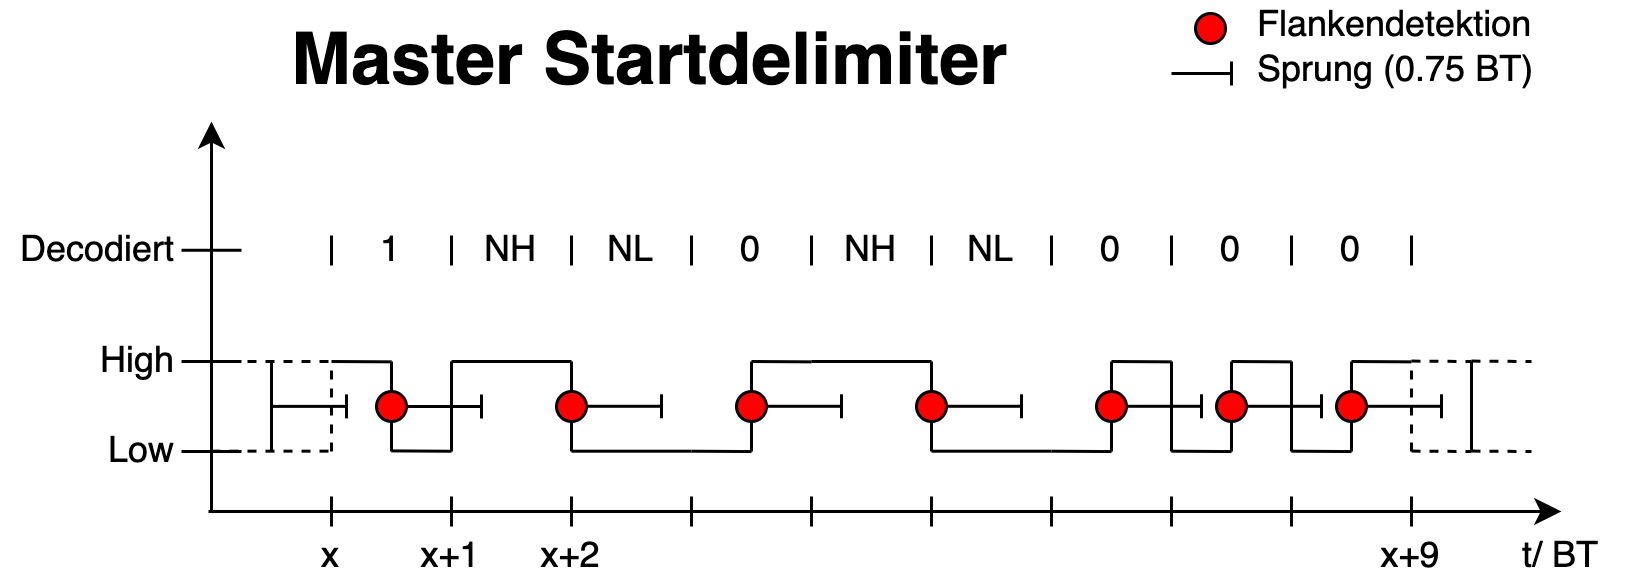
\includegraphics[width=\linewidth]{Figures/Chap3/Busauslastung/Master_Startdel.png}
    \caption{Anzahl Flanken in einem Master Startdelimiter ist 7}
    \label{fig:MasterStartdel}
\end{figure}

\begin{figure}[H]
    \centering
    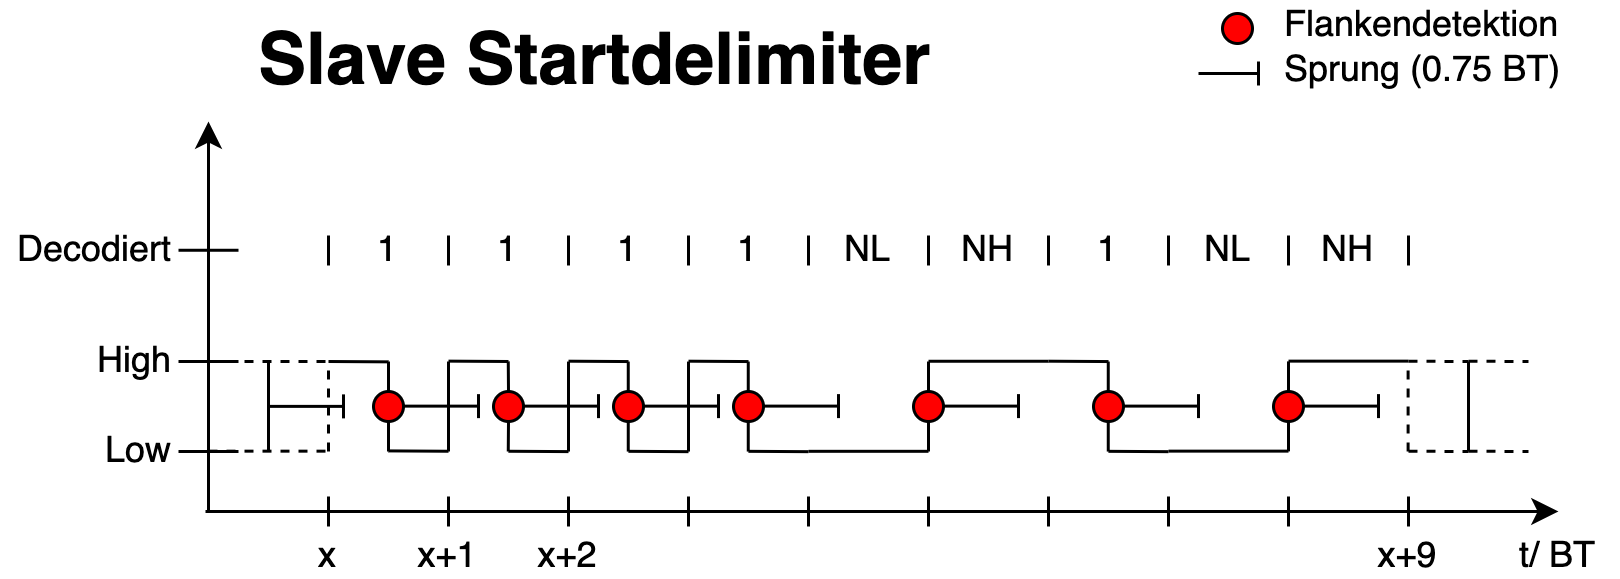
\includegraphics[width=\linewidth]{Figures/Chap3/Busauslastung/Slave_Startdel.png}
    \caption{Anzahl Flanken in einem Slave Startdelimiter ist 7}
    \label{fig:SlaveStartdel}
\end{figure}

\newpage
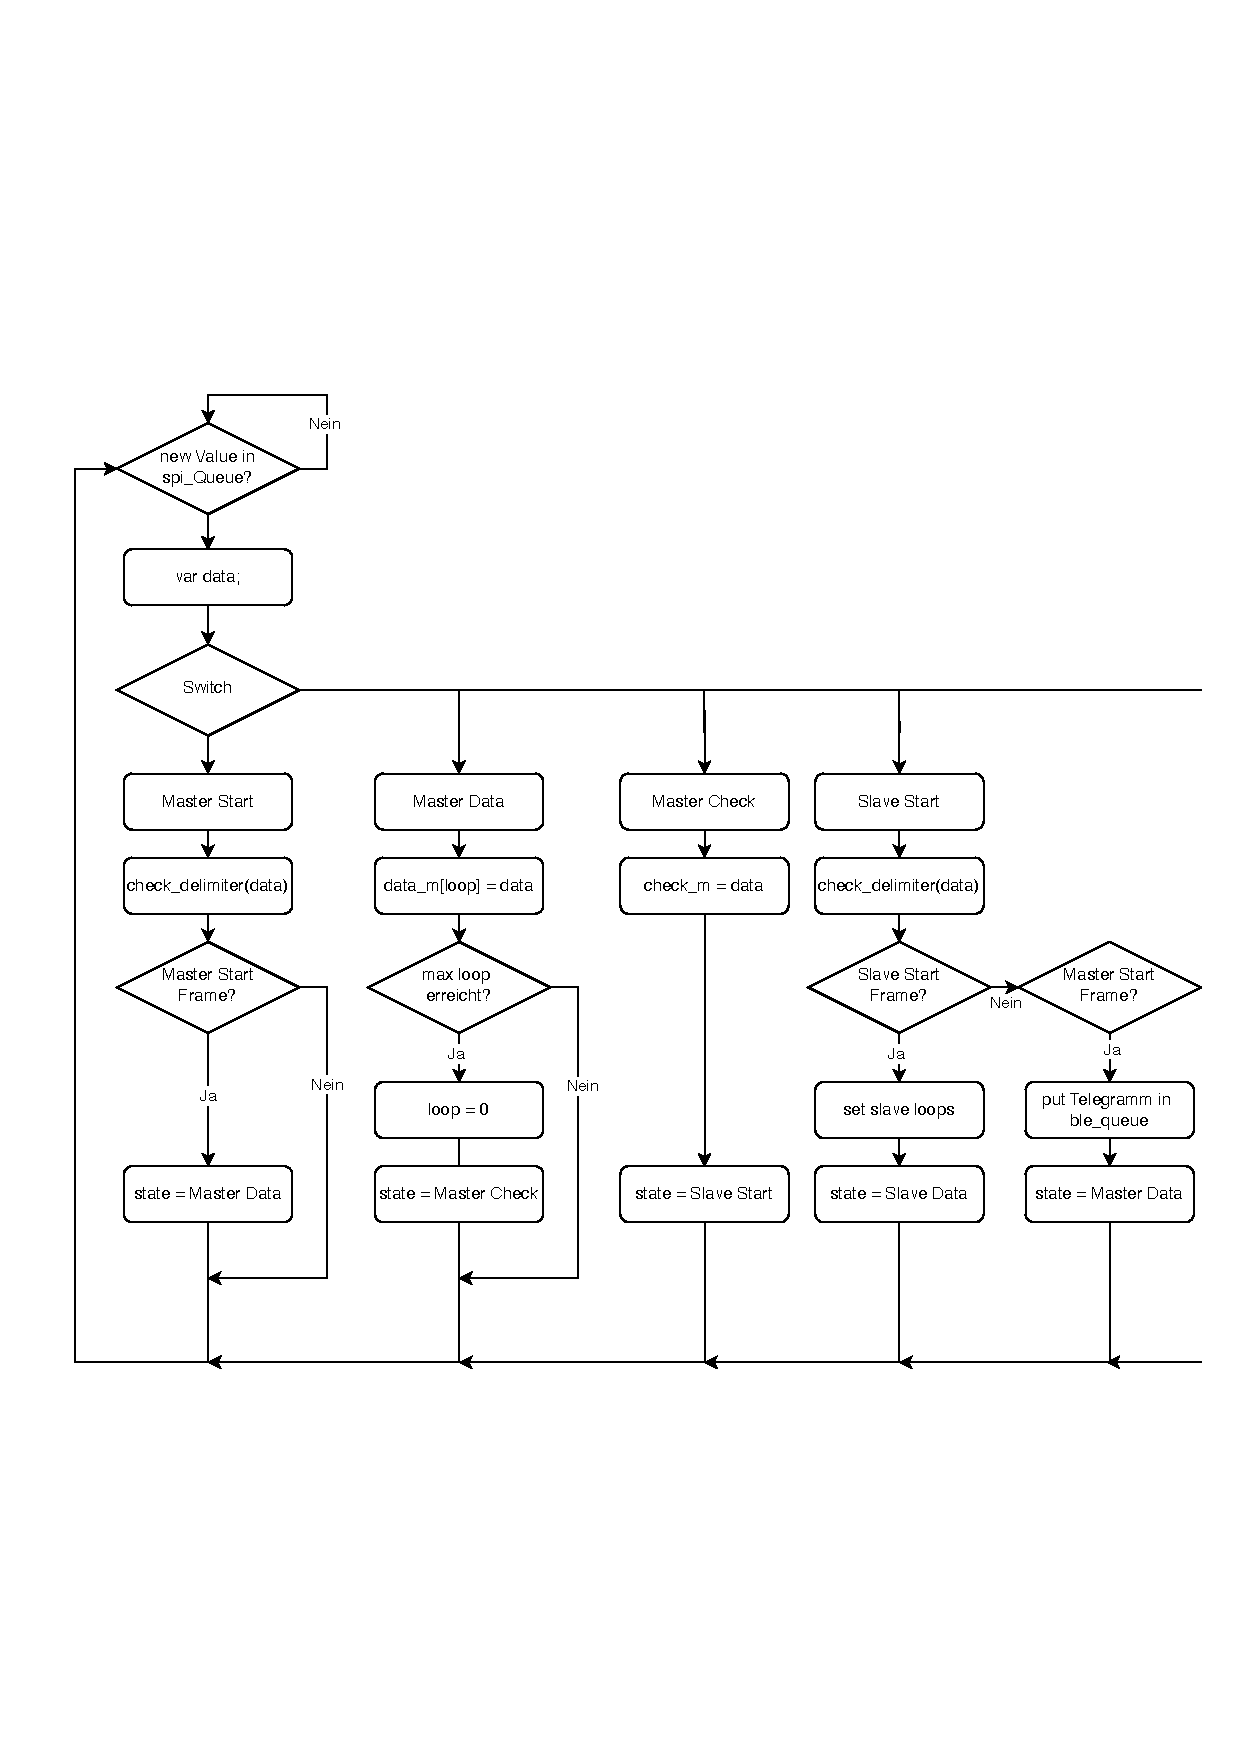
\includepdf[pages=1,pagecommand={\thispagestyle{headings} \section{Manchester Decoding State Machine} \label{app:ManchDec}}, scale=0.9]{Appendices/State_Machine_Manchester.pdf}


\includepdf[pages=2,pagecommand={\thispagestyle{headings}}, scale=0.9]{Appendices/State_Machine_Manchester.pdf}


\newpage
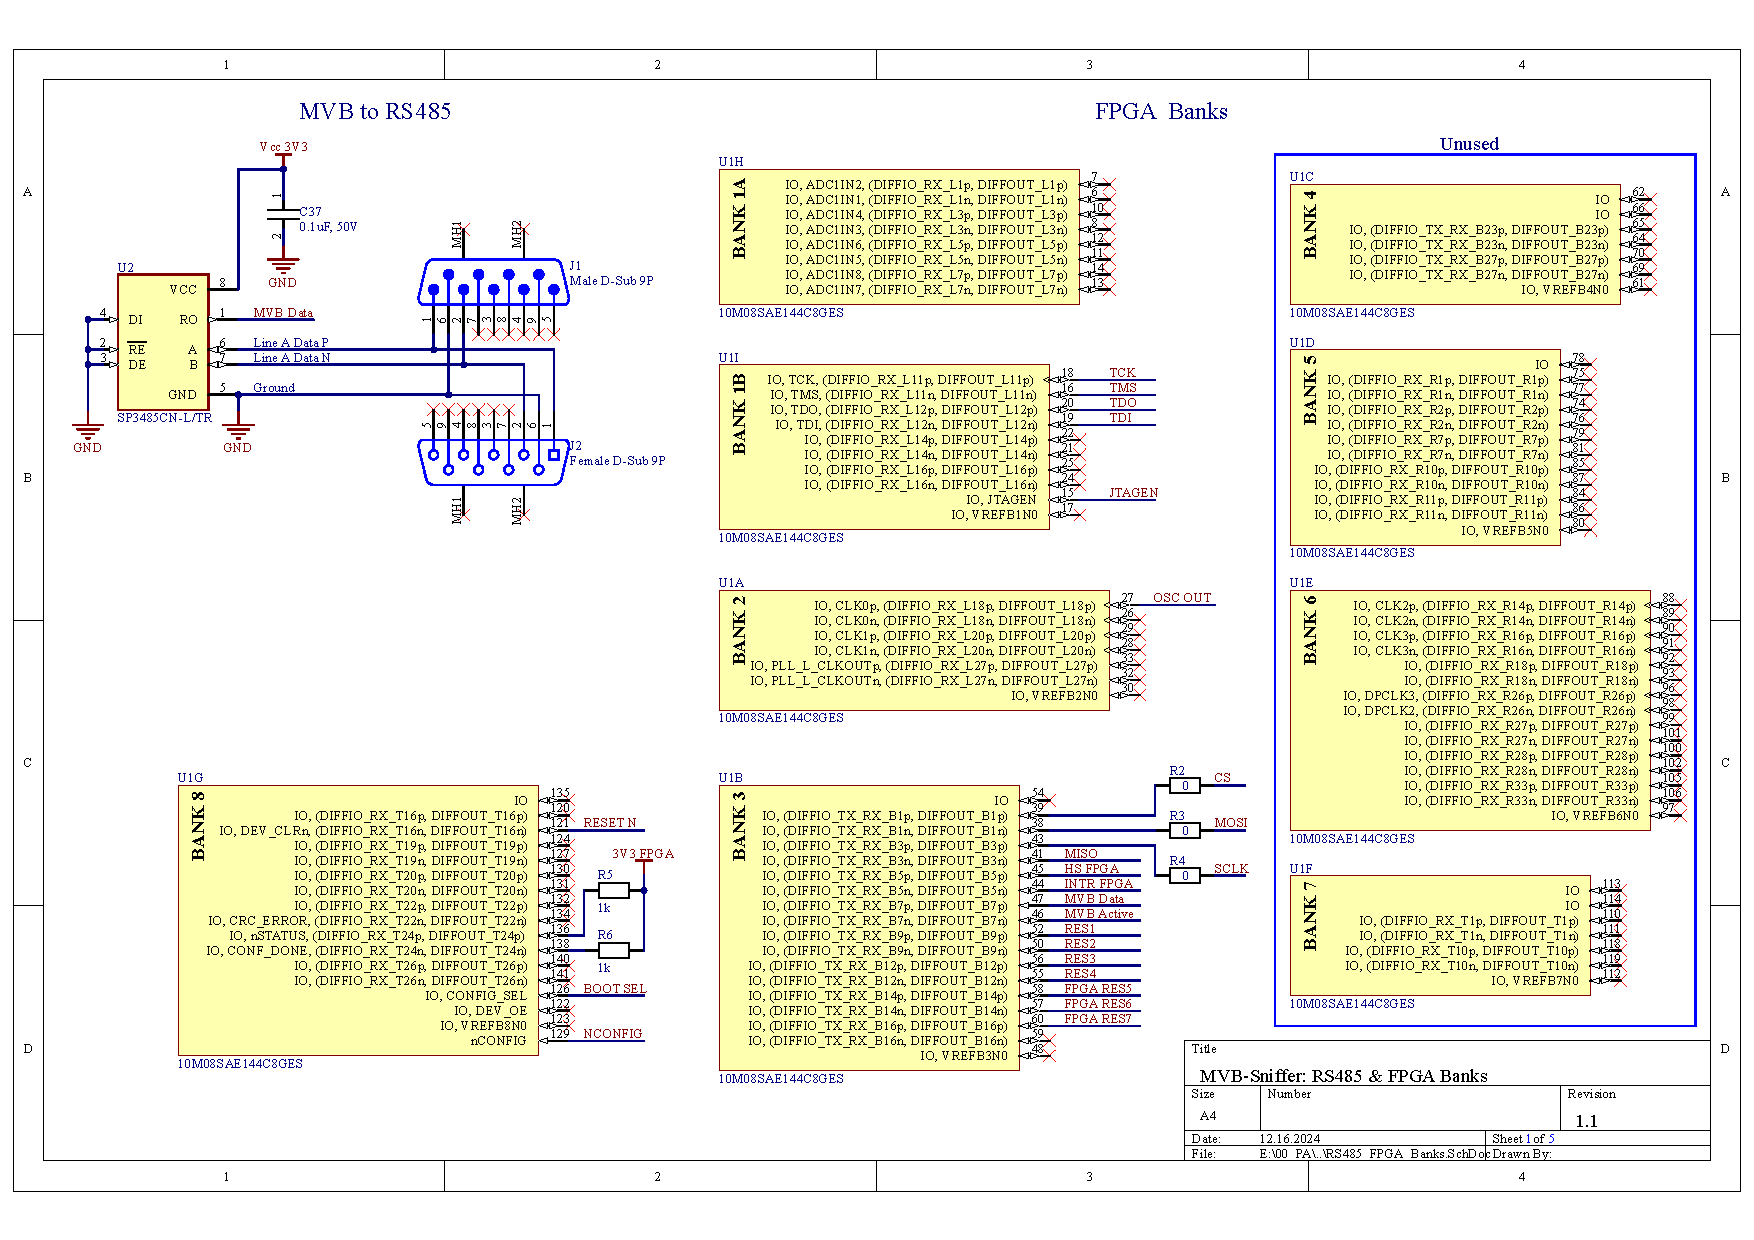
\includepdf[pages=1, angle=90,pagecommand={\thispagestyle{headings} \section{Schemata} \label{app:Schemata}}, scale=0.75]{Appendices/SchematicsV1_2.pdf}


\includepdf[pages=2, angle=90,pagecommand={\thispagestyle{headings}}, scale=0.8]{Appendices/SchematicsV1_2.pdf}

\includepdf[pages=3, angle=90,pagecommand={\thispagestyle{headings}}, scale=0.8]{Appendices/SchematicsV1_2.pdf}

\includepdf[pages=4, angle=90,pagecommand={\thispagestyle{headings}}, scale=0.8]{Appendices/SchematicsV1_2.pdf}

\includepdf[pages=5, angle=90,pagecommand={\thispagestyle{headings}}, scale=0.8]{Appendices/SchematicsV1_2.pdf}


\newpage
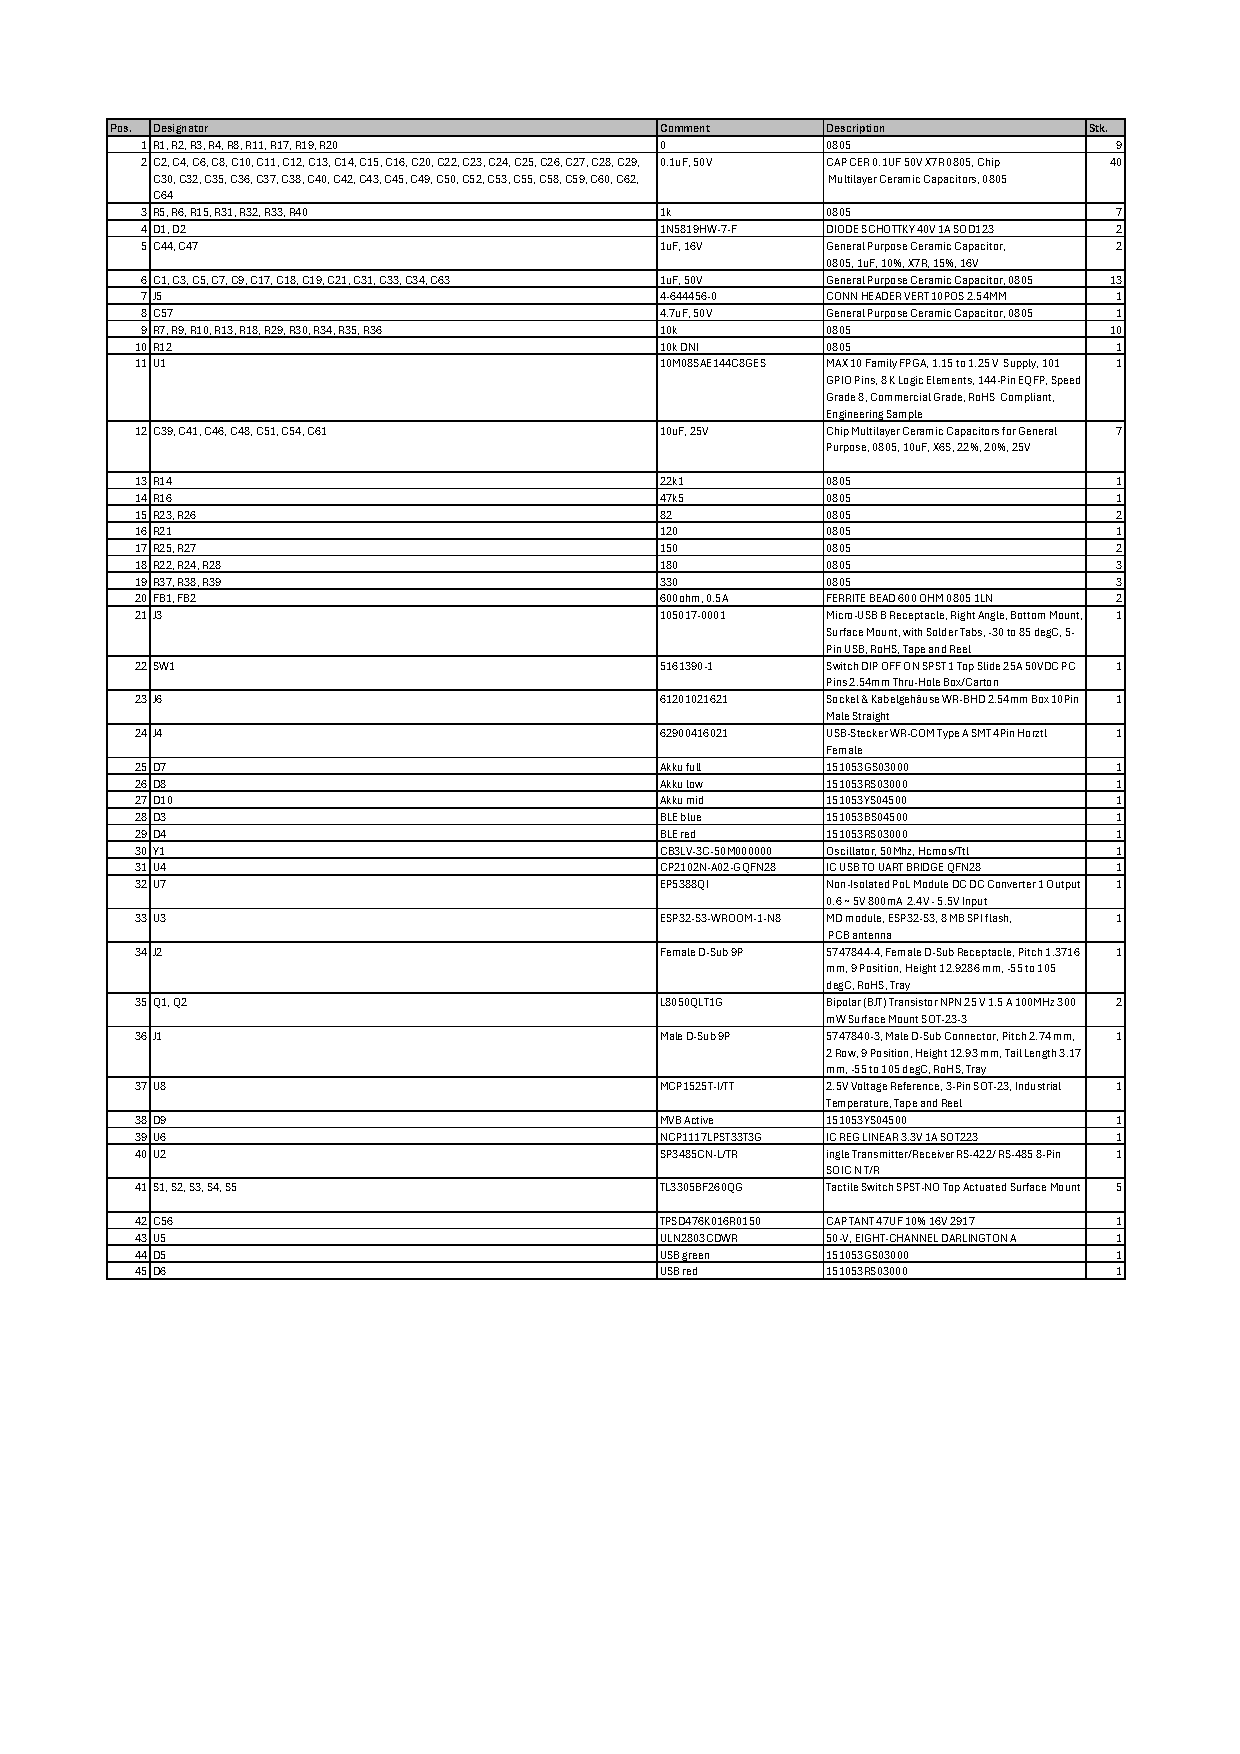
\includepdf[pages=1,pagecommand={\thispagestyle{headings} \section{Stückliste} \label{app:bom.pdf}}, scale=0.85]{Appendices/BOM_PCB_MVB_Sniffer.pdf}